\section{Experimental Evaluation}
Our experiments are organized into three parts. First, we describe the experimental setup and implementation details. Second, we evaluate the overall performance of OmniVTA on manipulation tasks involving diverse tactile interaction patterns. Then, we conduct comprehensive ablation studies to analyze the contribution of each module in the proposed policy.
Specifically, we investigate the following questions: 
(1) whether the TactileVAE can effectively encode tactile signals; 
(2) whether the proposed visuo-tactile world model can predict future tactile signals more accurately than alternative tactile prediction approaches; 
(3) whether incorporating predicted future tactile signals improves policy performance and whether the proposed usage of predicted tactile information in OmniVTA is effective; and 
(4) whether the Reflexive Latent Tactile Controller can generate reasonable fine-grained corrective actions and how much it improves policy execution. 
We further analyze the contribution of each design component through detailed ablation studies.

\subsection{Experimental Setup}

\begin{table*}[t]
\centering
\caption{Objects used for training and manipulation across different robotic tasks. Each object is associated with 150 manipulation trajectories in the dataset for training world models and manipulation policies.}
\small
\renewcommand{\arraystretch}{1.2}
\begin{tabular}{@{} l l l @{}}
\toprule
\textbf{Task} & \textbf{Object Used for Training} & \textbf{Object Used for Manipulation} \\
\midrule
\textbf{Wipe} & vases in 4 different colors and shapes, plate, and whiteboard  & vases in 4 different colors and shapes \\
\textbf{Peel} & cucumber, Chinese yam, radish, carrot, and white daikon & cucumber, Chinese yam, radish \\
\textbf{Cut} & cucumber, Chinese yam, carrot, pepper, and banana & cucumber, Chinese yam, pepper, banana \\
\textbf{Assembly} & 3 colors of USB stick and 3 types of charging adapters & red USB stick and silver USB stick \\
\textbf{Grasp} & blueberry, strawberry, grape, cherry, and cherry tomato & blueberry, strawberry, grape, and cherry tomato \\
\textbf{Adjustment} & test tube, pencil, cuboid, cylinder, and triangular prism & cuboid, cylinder \\
\bottomrule
\label{tab:object}
\end{tabular}
\vspace{-5mm}
\end{table*}

\subsubsection{Training Details}
Our OmniVTA framework is trained in four stages: training the TactileVAE, training the Visuo-Tactile World Model, training the Adaptive Visuo-Tactile Fusion Policy, and training the Reflexive Latent Tactile Controller.

\noindent\textbf{Training of TactileVAE.}
For training the TactileVAE, we use tactile data from 20\% of the manipulation trajectories, together with additional tactile interaction data collected from interactions between 10 extra objects and the tactile sensors. The resulting dataset contains approximately 1.2M tactile samples. 
Both TactileVAE and the VAE baselines are trained for 50 epochs using 8 NVIDIA A100 GPUs.
The loss weights are set to $\lambda_{\text{KL}}=1e-6$.

\noindent\textbf{Training of Visuo-Tactile World Model.}
We first construct a dataset to train the Visuo-Tactile World Model, comprising six categories of tactile interaction patterns. 
For each category, 5--6 objects are selected, and 150 manipulation trajectories per object are collected using TacUMI and the xArm7. 
The data are split into training and test sets with a 90\%/10\% ratio. 
A detailed breakdown of the dataset is provided in Table~\ref{tab:object}.

For training the Visuo-Tactile World Model, we use AdamW with a learning rate of $1\times10^{-4}$ and weight decay $0$. The per-GPU batch size is $5$, and the total number of training steps is $100{,}000$. The gradient norm threshold is set to $0.1$, with gradient clipping enabled after $20{,}000$ steps. The loss weights are set to $\lambda_{\text{dyn}}=1.0$ and $\lambda_{\text{amp}}=1.0$.

\noindent\textbf{Training of Adaptive Visuo-Tactile Fusion Policy.}
We used the same training set to train the Adaptive Visuo-Tactile Fusion Policy.
For each interaction category, the data are combined to train a unified visuo-tactile generation and manipulation model (OmniVTA), as well as other policy baselines. 
The Adaptive Visuo-Tactile Fusion Policy is trained for 250k steps. Other manipulation baselines are trained for 350k steps to compensate for the absence of additional perception modules.
The loss weights are set to $\lambda_{ct}=0.2$.

\noindent\textbf{Parameter settings.}
Following prior work, we adopt \emph{relative actions} as the action representation. 
During training, visual observations are sampled at 15\,Hz, tactile signals at 60\,Hz, and robot proprioception at 60\,Hz. 
The policy outputs action chunks at 15\,FPS. 
For observations, both OmniVTA and all baselines use the current and previous visual frames (2 frames in total), the corresponding 8 tactile frames within the same temporal window, and 2 proprioceptive observations as policy inputs. 
Each action chunk predicts the next 6 actions, which are interpolated to 60\,Hz during execution.

\subsubsection{Hardware Setup}

The experimental platform consists of a UFactory xArm7 robotic arm equipped with a parallel two-finger gripper and two fingertip tactile sensors. 
An Intel RealSense D435 camera mounted on the robot wrist provides RGB observations at 15\,Hz, while the tactile sensors capture tactile signals at 60\,Hz. For the TactileVAE validation experiments, three types of tactile sensors are used: GelSight Mini, Tac3D, and Xense. 
The resolutions of their reconstructed 3D displacement fields are $7\times9$, $20\times20$, and $35\times20$, respectively. 
In the real-world manipulation experiments, we use only the Xense sensors.

\subsubsection{Baselines}
We select representative baseline methods to evaluate the effectiveness of the proposed TactileVAE, Visuo-Tactile World Model, and the overall OmniVTA framework. 

\noindent \textbf{TactileVAE baselines.} We compare the proposed TactileVAE with two representative tactile encoding methods: PCA-based features and a point cloud-based autoencoder~\cite{chen2024general}.

\noindent \textbf{Tactile prediction baselines.}
We compare our Visuo-Tactile World Model against three representative paradigms for multi-modal generative modeling.

\begin{itemize}
\item \textbf{Unified multimodal generation}:
UVA~\cite{li2025unified} models video frames and actions as a unified token sequence and jointly generates them using a single generative model. We extend this formulation by injecting tactile tokens.

\item \textbf{Joint trajectory diffusion}:
ForceMimic~\cite{liu2025forcemimic} and KineDex~\cite{zhang2025kinedex} concatenate interaction forces with actions and learn diffusion-based policies conditioned on visual observations. In our implementation, we replace force inputs with tactile feature embeddings extracted using a lightweight MLP autoencoder.

\item \textbf{Conditional modality prediction}:
exUMI~\cite{xu2025exumi} generates future tactile signals using a latent diffusion model (LDM) conditioned on visual observation and action. Since our method assumes only historical observations are available at inference, future action inputs are replaced with historical action sequences.
\end{itemize}

\noindent \textbf{Contact-rich policy baselines.}
We compare against several state-of-the-art imitation learning policies:

\begin{itemize}
\item \textbf{DP}~\cite{chi2025diffusion}: Diffusion Policy using wrist-view RGB observations and open-loop action chunk execution.
\item \textbf{DP+tactile}: Diffusion Policy augmented with tactile features encoded by PCA.
\item \textbf{KineDex}~\cite{zhang2025kinedex}: a diffusion policy that jointly predicts actions and forces from visual observations.
\item \textbf{ForceMimic}~\cite{liu2025forcemimic}: a diffusion policy conditioned on 3D observations that jointly predicts actions and forces.
\item \textbf{RDP}~\cite{xue2025reactive}: a reactive diffusion policy with a slow diffusion planner and a fast tactile-based reactive controller.
\item \textbf{OmniVTA (ours)}: our method with a visuo-tactile world model and a dual-system manipulation policy consisting of a diffusion planner and a reflexive tactile controller.
\item \textbf{OmniVTA w/o RLTC}: our method without the reflexive controller, executing diffusion-planned action chunks in a open-loop manner.
\end{itemize}

\begin{figure}[ht]
\centering
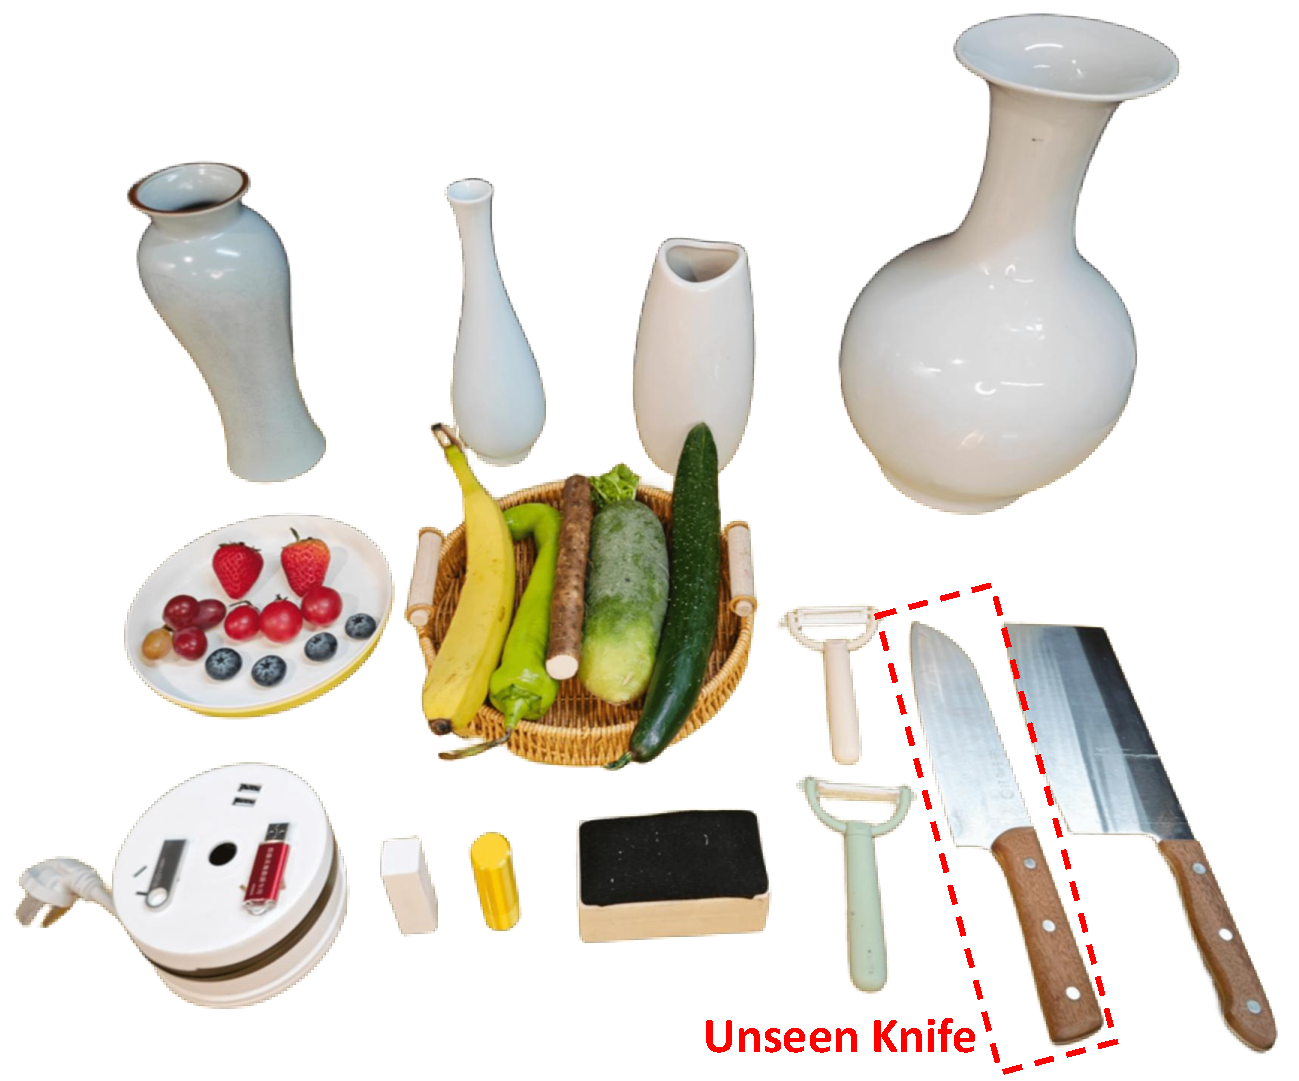
\includegraphics[width=0.75\linewidth]{fig/object.pdf}
\caption{\textbf{Objects used in the manipulation tasks.}}
\label{fig:object}
\vspace{-3mm}
\end{figure}

\subsection{Overall Performance}

We evaluate the real-world manipulation performance of OmniVTA from three perspectives: object diversity, generalization, and perturbation robustness.

\noindent \textbf{Object diversity.}
For each category, we evaluate the policy on 2--4 different objects, as summarized in Table~\ref{tab:object} and Fig.~\ref{fig:object}. 
Before each trial, the object is placed at a random position and fixed during manipulation. 
For each object, we perform 10 trials and report the average success rate.

\noindent \textbf{Generalization.}
We evaluate two types of generalization.

(1) \emph{Position generalization.}
For the wipe, peel, assembly, and adjustment tasks, objects are placed at two additional unseen heights during evaluation. 
For each object and each height, we conduct 5 trials and report the average success rate.

(2) \emph{Tool generalization.}
For the cut task, we replace the training knife with a previously unseen knife (shown in Fig.~\ref{fig:object}). 
Each object is tested 10 times using the new tool.


\noindent \textbf{Perturbation robustness.}
For the wipe, peel, cut, and assembly tasks, we introduce controlled perturbations during execution to disrupt the current contact state. 
Specifically, the target object is suddenly displaced upward or downward along the vertical direction during the interaction phase. 
This perturbation breaks the existing contact state and requires the policy to re-establish stable contact. 
For each task, one representative object is selected and evaluated over 10 trials.

\noindent \textbf{Evaluation metric.}
The primary evaluation metric is task success rate. 
A trial is considered successful if the task objective is completed and no damage occurs to the tactile sensors during execution. For wiping, peeling, and cutting tasks, we measure task completion using the ratio of the successfully processed length (e.g., the proportion of removed peel, erased marks, or completed cuts). For assembly and grasping tasks, a trial is considered successful only if the object is fully inserted or grasped without damage. For adjustment tasks, success is defined as achieving a pose change that exceeds a predefined angular threshold (60°).

\noindent \textbf{Results.}
The overall real-robot manipulation results are visualized in Fig.~\ref{fig:manipulation}, and the corresponding overall success rates are reported in Table~\ref{tab:full_comparison_final_scaled}.
In the object diversity evaluation, OmniVTA achieves the best performance across all six tasks, demonstrating the effectiveness of the proposed framework. 
Adding the closed-loop controller further improves performance compared with the open-loop variant (OmniVTA w/o RLTC), highlighting the importance of feedback control in contact-rich manipulation.

\begin{figure*}[t]
\centering
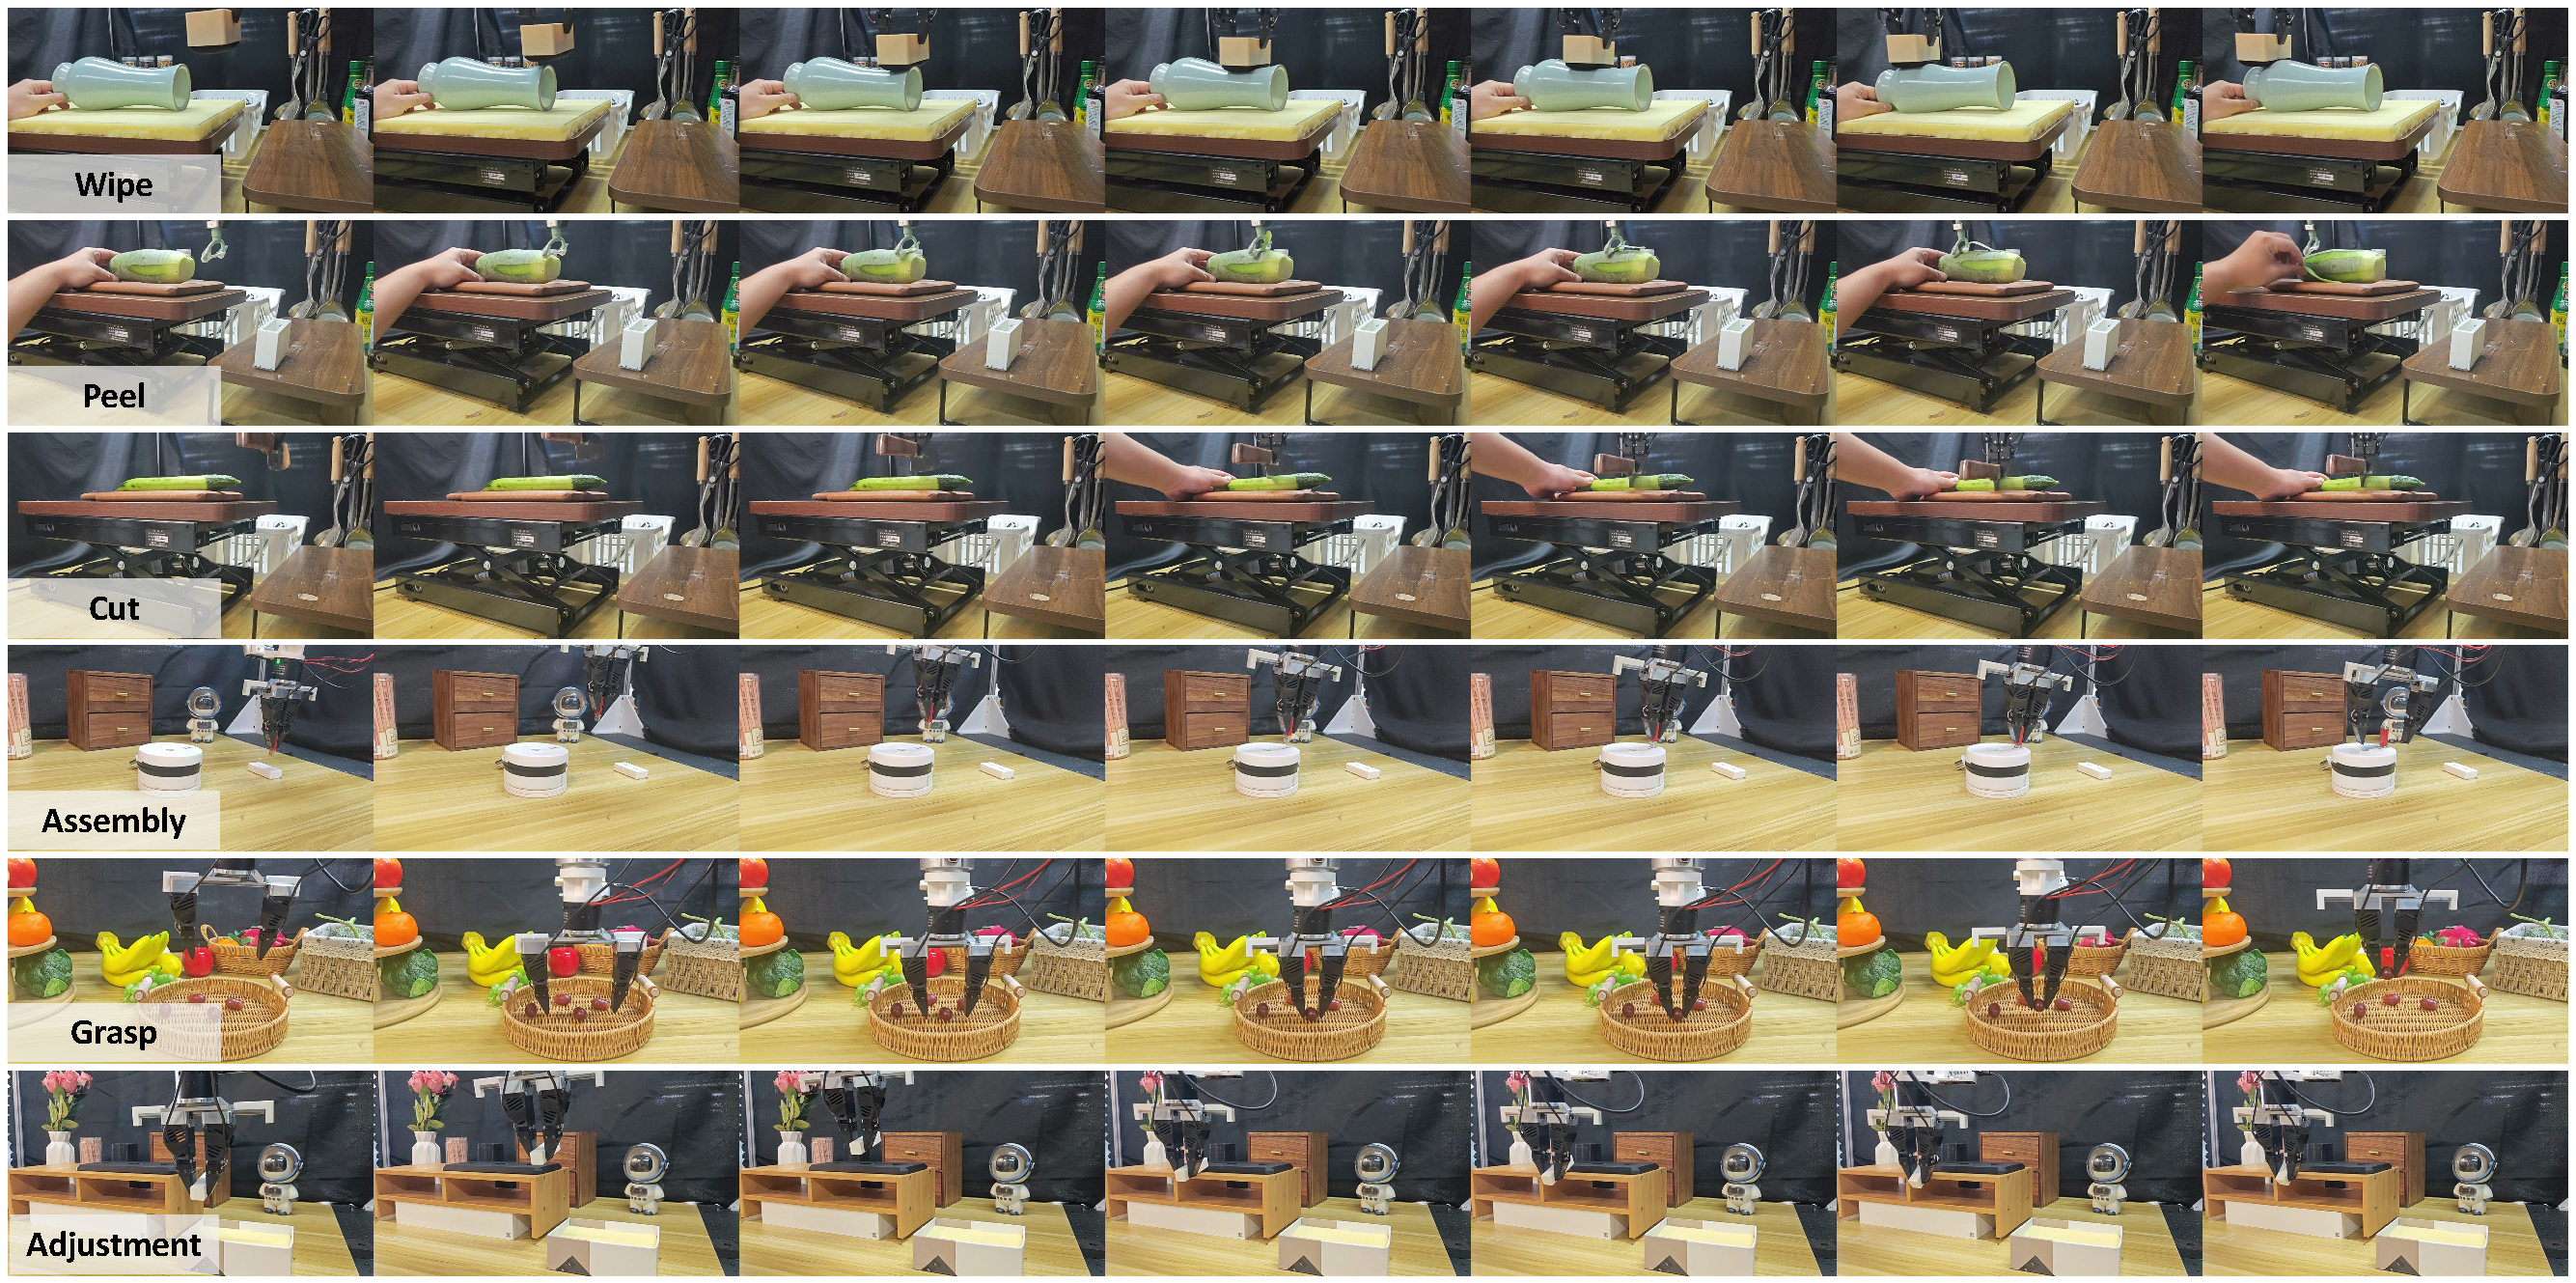
\includegraphics[width=0.95\linewidth]{fig/manipulation.pdf}
\caption{\textbf{Real-robot manipulation results.} We visualize the manipulation process across six task categories.}
\label{fig:manipulation}
\end{figure*}

\begin{table*}[t]
\centering
\caption{Performance comparison of OmniVTA and baseline methods across six tasks under three evaluation settings: object diversity (O), generalization (G), and perturbation robustness (P). Results are reported in terms of success rate.}
\label{tab:full_comparison_final_scaled}
\small
\setlength{\tabcolsep}{2.5pt}
\renewcommand{\arraystretch}{1.3}

\begin{tabularx}{\textwidth}{@{} l *{15}{>{\centering\arraybackslash}X} @{}}
\toprule
\textbf{Task} & \multicolumn{3}{c}{\textbf{Wipe}} & \multicolumn{3}{c}{\textbf{Peel}} & \multicolumn{3}{c}{\textbf{Cut}} & \multicolumn{3}{c}{\textbf{Assembly}} & \multicolumn{1}{c}{\textbf{Grasp}} & \multicolumn{2}{c}{\textbf{Adjustment}} \\
\cmidrule(lr){2-4} \cmidrule(lr){5-7} \cmidrule(lr){8-10} \cmidrule(lr){11-13} \cmidrule(lr){14-14} \cmidrule(lr){15-16}
\makecell[l]{\textbf{Method /}\textbf{ Eval. setting}} & \textbf{O} & \makecell[c]{{\textbf{G}}} & \textbf{P} & \textbf{O} & \makecell[c]{\textbf{G}} & \textbf{P} & \textbf{O} & \makecell[c]{{\textbf{G}}} & \textbf{P} & \textbf{O} & \makecell[c]{{\textbf{G}}} & \textbf{P} & \textbf{O} & \textbf{O} & \makecell[c]{\textbf{G}} \\
\midrule
DP               & 0.12 & 0.05 & 0 & 0.06 & 0 & 0 & 0.28 & 0.10 & 0 & 0.10 & 0 & 0.05 & 0.20 & 0 & 0 \\
DP+tactile       & 0.36 & 0.28 & 0 & 0.32 & 0.20 & 0.08 & 0.33 & 0.15 & 0.13 & 0.30 & 0.10 & 0.10 & 0.48 & 0.25 & 0.15 \\
KineDex          & 0.40 & 0.25 & 0 & 0.24 & 0.13 & 0.05 & 0.38 & 0.30 & 0.20 & 0.30 & 0.15 & 0.15 & 0.65 & 0.30 & 0.20 \\
ForceMimic       & 0.33 & 0.20 & 0 & 0.27 & 0.18 & 0 & 0.50 & 0.25 & 0.05 & 0.35 & 0.15 & 0.10 & 0.60 & 0.10 & 0 \\
RDP              & 0.50 & 0.38 & 0.42 & 0.48 & 0.36 & 0.45 & 0.65 & 0.50 & 0.43 & \textbf{0.60} & \textbf{0.50} & 0.35 & 0.88 & 0.50 & 0.50 \\
OmniVTA w/o RLTC & 0.66 & 0.40 & 0.25 & 0.40 & 0.30 & 0.20 & 0.50 & 0.50 & 0.20 & 0.40 & 0.35 & 0.20 & 0.70 & 0.40 & 0.30 \\
\textbf{OmniVTA} & \textbf{0.80} & \textbf{0.58} & \textbf{0.60} & \textbf{0.55} & \textbf{0.48} & \textbf{0.63} & \textbf{0.85} & \textbf{0.83} & \textbf{0.60} & \textbf{0.60} & \textbf{0.50} & \textbf{0.40} & \textbf{0.90} & \textbf{0.65} & \textbf{0.65} \\
\bottomrule
\end{tabularx}
\vspace{-3mm}
\end{table*}

We also observe that, for contact-rich tasks involving strong physical interactions (e.g., wiping, peeling, cutting), the performance gain from the reactive policy in RDP (compared with DP+tactile) is smaller than the improvement brought by our reflexive controller.
This is because our controller leverages predicted tactile signals as targets to regulate the robot's motion, enabling reliable contact while preventing excessive contact forces. 
During the contact phase, the average tangential deformation measured by our tactile sensors is 0.35 with a maximum of 0.72. 
In contrast, the reactive policy in RDP often produces overly strong contacts that damage the sensors, with an average deformation of 0.56 and a maximum of 1.1. In the unseen-height evaluation, the performance of RDP drops moderately, while other baselines degrade significantly. 
In contrast, OmniVTA without the closed-loop controller already surpasses RDP, indicating stronger robustness to geometric variations. In the tool generalization experiment, replacing the knife with a smaller, unseen tool has little impact on our performance in the cut task. 
This suggests that the policy relies on tactile feedback rather than memorizing demonstration trajectories. Finally, in the perturbation experiments, OmniVTA consistently achieves the highest success rates. 
Moreover, the closed-loop controller significantly improves performance compared with the open-loop variant, demonstrating its ability to quickly recover stable contact during perturbations.

\vspace{-3mm}
\subsection{Component Analysis}
\subsubsection{TactileVAE}
We evaluate TactileVAE from two aspects: reconstruction accuracy and latent representation quality.

\noindent \textbf{Reconstruction evaluation.}
We compare TactileVAE with baseline methods across six categories of tactile interaction patterns. 
Reconstruction performance is evaluated using the $L_2$ distance and cosine similarity, which measure the magnitude and directional consistency of the reconstructed 3D deformation, respectively. 
The $L_2$ metric is computed over the entire deformation field, while cosine similarity is computed over non-zero deformation regions only. 
As shown in Table~\ref{tab:vae}, the proposed TactileVAE consistently achieves the best performance across all six categories, demonstrating its effectiveness in modeling tactile deformation.

\begin{table*}[t]
\centering
\caption{Performance comparison of different methods across robotic tasks using L2 and cosine similarity metrics. Lower L2 ($\downarrow$) and higher cos ($\uparrow$) indicate better performance.}
\label{tab:vae}
\small 
\renewcommand{\arraystretch}{1.2}

\begin{tabular*}{\textwidth}{@{\extracolsep{\fill}} l ccccc ccccc cc}
\toprule
\textbf{Method} & \multicolumn{2}{c}{\textbf{Wipe}} & \multicolumn{2}{c}{\textbf{Peel}} & \multicolumn{2}{c}{\textbf{Cut}} & \multicolumn{2}{c}{\textbf{Assembly}} & \multicolumn{2}{c}{\textbf{Grasp}} & \multicolumn{2}{c}{\textbf{Adjustment}} \\
\cmidrule(lr){2-3} \cmidrule(lr){4-5} \cmidrule(lr){6-7} \cmidrule(lr){8-9} \cmidrule(lr){10-11} \cmidrule(lr){12-13}
& {L2 $\downarrow$} & {cos $\uparrow$} & {L2 $\downarrow$} & {cos $\uparrow$} & {L2 $\downarrow$} & {cos $\uparrow$} & {L2 $\downarrow$} & {cos $\uparrow$} & {L2 $\downarrow$} & {cos $\uparrow$} & {L2 $\downarrow$} & {cos $\uparrow$} \\
\midrule
PCA         & 0.091 & 0.810 & 0.085 & 0.430 & 0.109 & 0.400 & 0.071 & 0.720 & 0.036 & 0.600 & 0.069 & 0.560 \\
PointNet-AE & 0.059 & 0.910 & 0.067 & 0.850 & 0.062 & 0.840 & 0.058 & 0.900 & 0.028 & \textbf{0.750} & 0.047 & 0.760 \\
\textbf{Ours} & \textbf{0.038} & \textbf{0.930} & \textbf{0.033} & \textbf{0.880} & \textbf{0.031} & \textbf{0.940} & \textbf{0.022} & \textbf{0.910} & \textbf{0.011} & 0.720 & \textbf{0.017} & \textbf{0.850} \\
\bottomrule
\end{tabular*}
\end{table*}

\noindent \textbf{Latent representation analysis.}
To further evaluate the learned tactile representations, we conduct experiments on three unseen objects under three types of force patterns (press, twist, and slide) using three tactile sensors, two of which are unseen during training, as shown in Fig.~\ref{fig:vae_tsne}(a) and (b). 
We record the tactile signals and extract their features using several variants of TactileVAE, including:
\begin{itemize}
    \item \textbf{w/o implicit decoder:} decodes the latent feature map without query-based sampling and query points input.
    \item \textbf{w/ position embedding:} incorporates positional encoding during decoding.
    \item \textbf{w/o spatial feature map:} represents the latent as a single token and decodes it with an implicit decoder.
    \item \textbf{w/ implicit decoder:} decodes the latent feature map via an implicit decoder.
\end{itemize}
All models are trained using only 5\% of the tactile dataset.

For visualization, the spatio-temporal tactile features are aggregated via max pooling to obtain sequence-level embeddings, which are then visualized using t-SNE. 
As shown in Fig.~\ref{fig:vae_tsne}(c), the learned representations exhibit clear clustering across different force patterns, even under cross-sensor settings. 
In contrast, marker-based encoding and variants without positional information fail to produce well-separated clusters, highlighting the importance of implicit neural representations for learning discriminative tactile features.

Finally, we compare two forms of tactile feature representations: local feature maps (patch-based features) and a global token obtained via max pooling. 
As shown in Fig.~\ref{fig:vae_tsne}(c) and Table~\ref{tab:vae_ablation}, local feature maps achieve better reconstruction accuracy and yield more informative tactile embeddings than the global token representation.

\begin{table}[t]
\centering
\caption{Ablation study on the design of TactileVAE. We evaluate reconstruction performance using the $L_2$ metric.}
\label{tab:vae_ablation}
\small
\renewcommand{\arraystretch}{1.2} % 增加行间距，提升阅读舒适度
% 设置列间距，让1栏宽度的表格看起来更紧凑
\setlength{\tabcolsep}{2pt} 

\begin{tabular}{l S[table-format=1.3] S[table-format=1.3] S[table-format=1.3]}
\toprule
\textbf{Method} & {\textbf{GelSight-Mini}} & {\textbf{Tac3D-A1}} & {\textbf{Xense-QN1}} \\
\midrule
w/o implicit decoder & 0.126 & 0.098 & 0.038 \\
w/ position embed. & 0.102 & 0.085 & 0.035 \\
w/o spatial feature map & 0.107 & 0.084 & 0.071 \\
w/ implicit decoder & \textbf{0.047} & \textbf{0.058} & \textbf{0.034} \\
\bottomrule
\end{tabular}
\end{table}

\begin{figure}[ht]
\centering
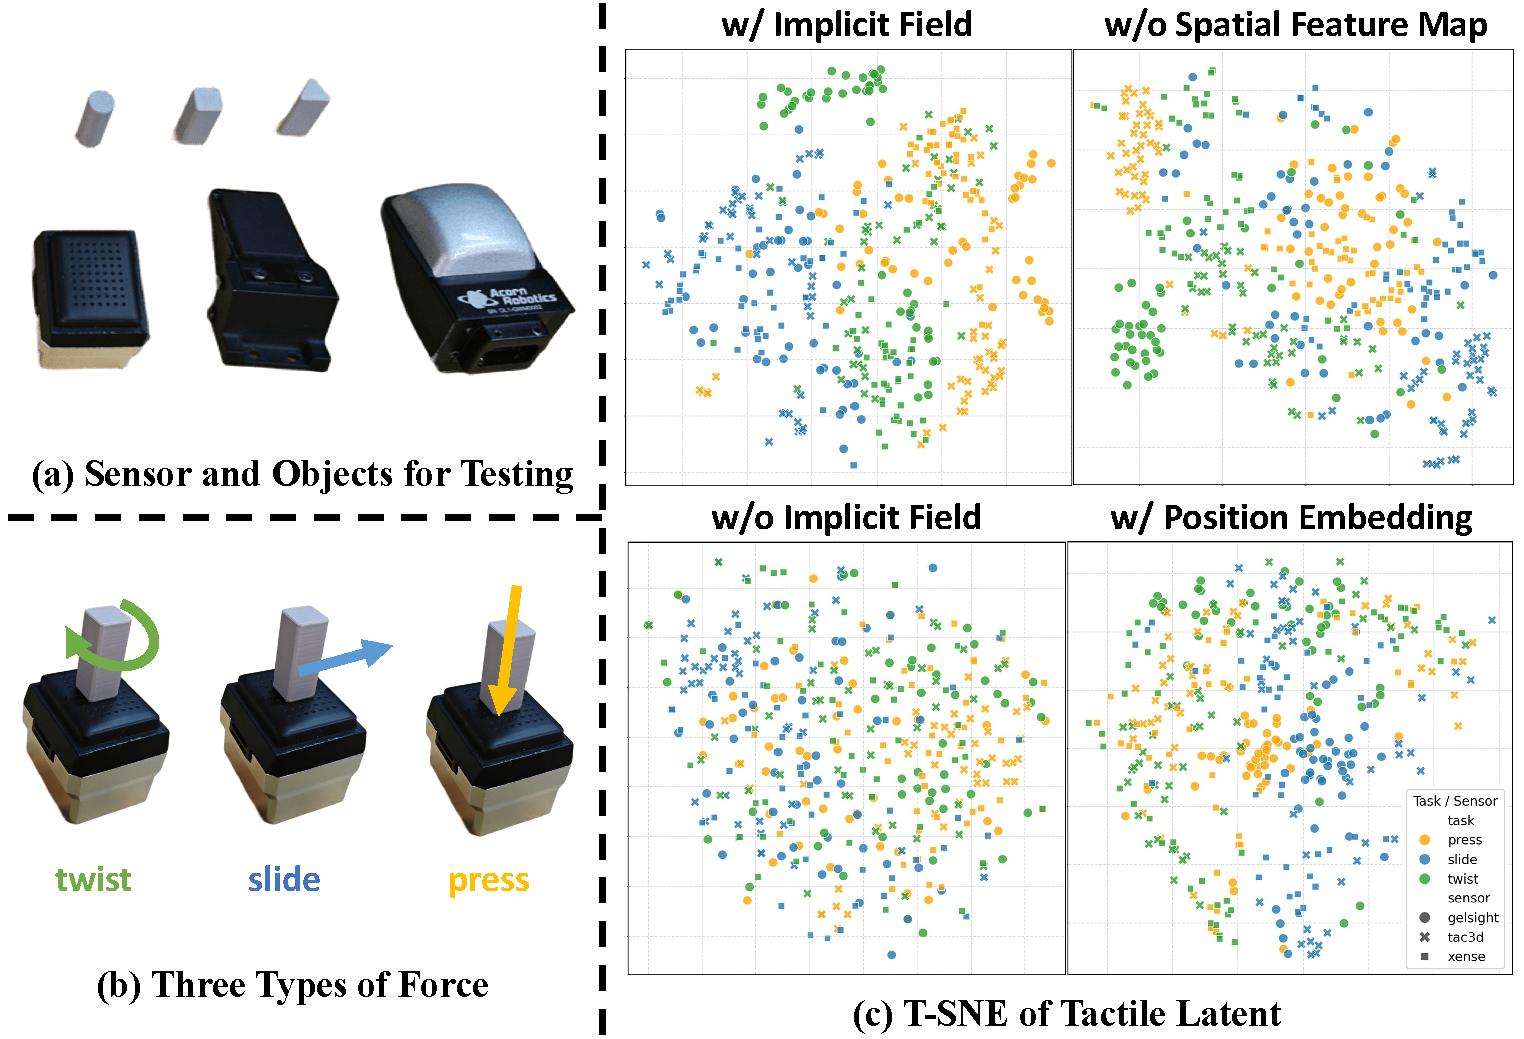
\includegraphics[width=\linewidth]{fig/tsne.pdf}
\caption{\textbf{Ablation study of TactileVAE.}\textbf{(a)} shows the sensors and objects for testing. \textbf{(b)} represents the three types of force loaded on the sensors. \textbf{(c)} visualizes the t-SNE of the tactile latent feature maps extracted by different models.}
\label{fig:vae_tsne}
\vspace{-3mm}
\end{figure}

\subsubsection{Visuo-Tactile World Model}

\begin{figure*}[ht]
\centering
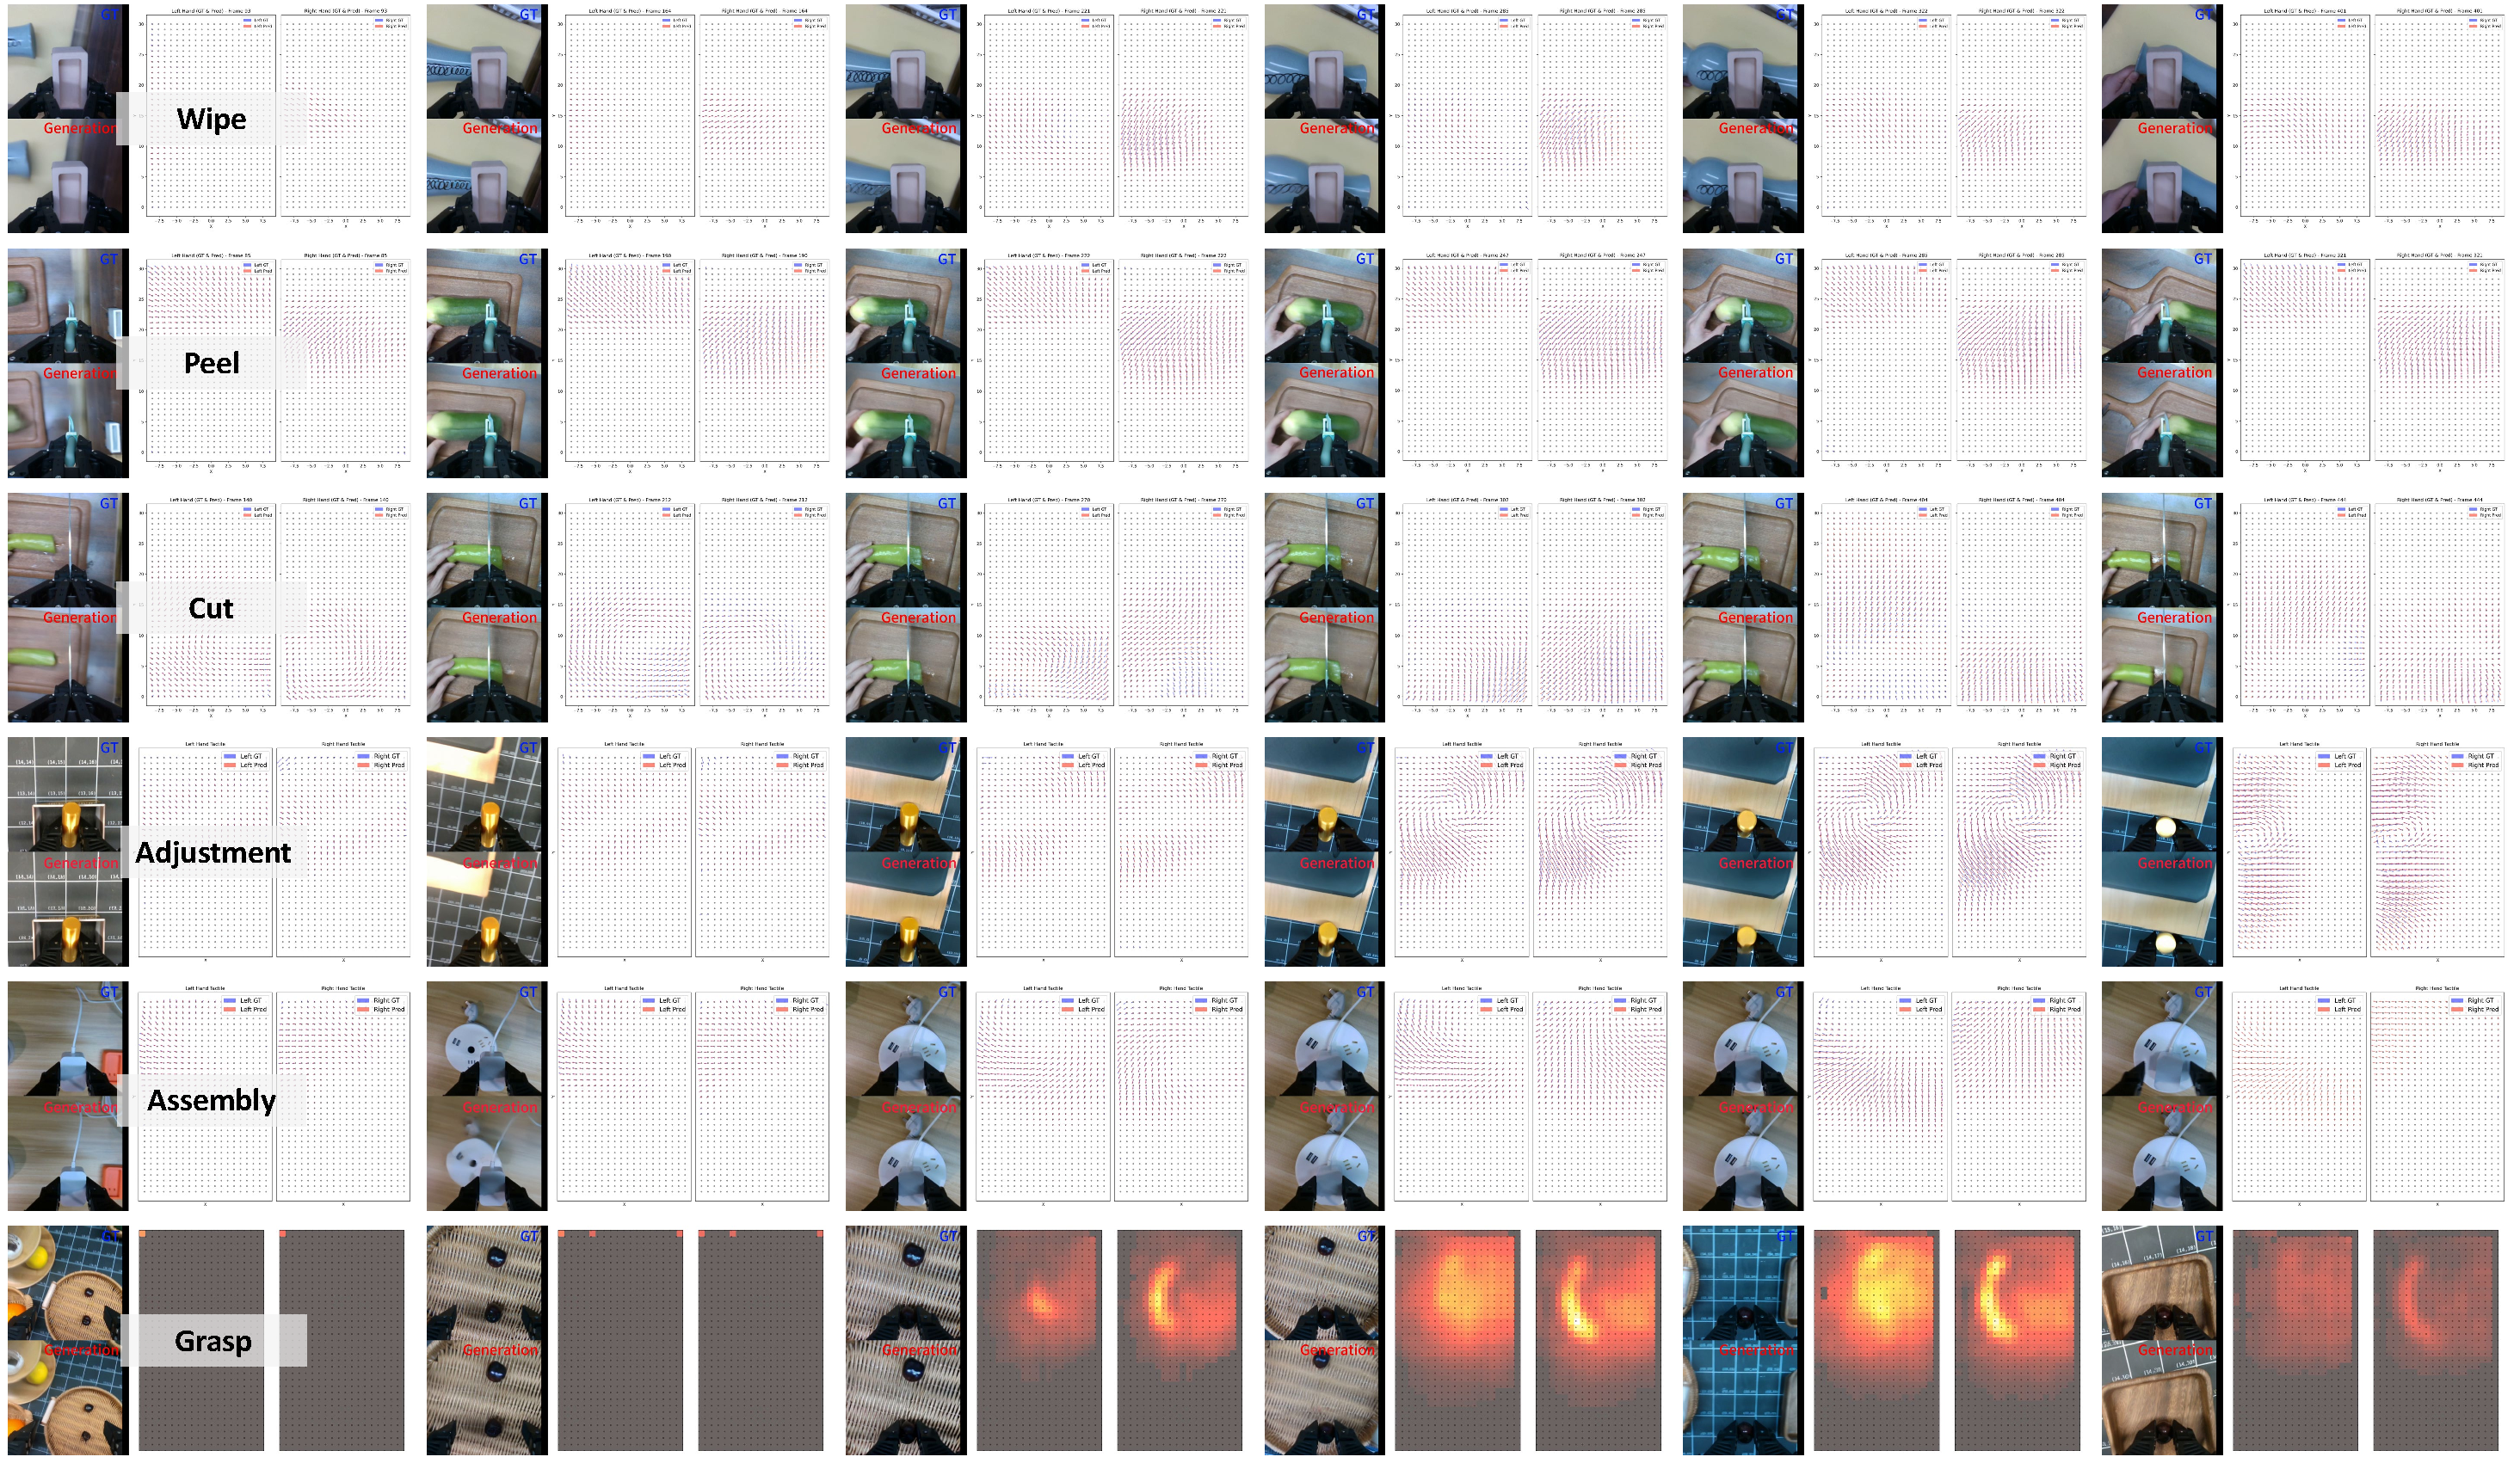
\includegraphics[width=\linewidth]{fig/wm.pdf}
\caption{\textbf{Visuo-tactile generation visualization across six task categories.} Red arrows indicate predicted tangential deformation, while blue arrows denote ground truth. Normal deformation in the grasp task is visualized using heatmaps. }
\label{fig:wm}
\end{figure*}

% 需要的宏包（如果你还没引入）：
% \usepackage{graphicx}   % for \resizebox
% \usepackage{multirow}   % 可选
% \usepackage{amsmath}    % 可选（数学下标更舒服）

% =========================
% Row 1: wipe / peel / cut
% =========================
\begin{table*}[t]
\centering
\scriptsize
\setlength{\tabcolsep}{2pt}
\renewcommand{\arraystretch}{1.15}
\caption{Prediction performance. We report the $L_2$ distance and cosine similarity at the 2nd, 4th, and 6th latent prediction steps (denoted as $L2_1, L2_2, L2_3$ and $C_1, C_2, C_3$), corresponding to the 8th, 16th, and 24th decoded tactile frames, respectively. We also report the average performance over all 24 predicted frames ($L2_{\text{avg}}$, $C_{\text{avg}}$). Top: Wipe/Peel/Cut. Bottom: Adjustment/Assembly/Grasp. ``--" denotes not applicable.}
\label{tab:wm_exp}
\resizebox{\textwidth}{!}{%
\begin{tabular}{l|cccccccc|cccccccc|cccccccc}
\hline
\multicolumn{1}{c|}{} &
\multicolumn{8}{c|}{\textbf{Wipe}} &
\multicolumn{8}{c|}{\textbf{Peel}} &
\multicolumn{8}{c}{\textbf{Cut}} \\
\hline
\textbf{Method} &
$L2_1$ & $L2_2$ & $L2_3$ & $L2_{\text{avg}}$ & $C_1$ & $C_2$ & $C_3$ & $C_{\text{avg}}$ &
$L2_1$ & $L2_2$ & $L2_3$ & $L2_{\text{avg}}$ & $C_1$ & $C_2$ & $C_3$ & $C_{\text{avg}}$ &
$L2_1$ & $L2_2$ & $L2_3$ & $L2_{\text{avg}}$ & $C_1$ & $C_2$ & $C_3$ & $C_{\text{avg}}$ \\
\hline
\textbf{UVA} &
0.084 & 0.091 & 0.088 & 0.088 & 0.68 & 0.65 & 0.64 & 0.66 &
0.090 & 0.097 & 0.102 & 0.097 & 0.62 & 0.60 & 0.60 & 0.61 &
0.075 & 0.076 & 0.078 & 0.077 & 0.72 & 0.71 & 0.71 & 0.71 \\

\textbf{exUMI} &
0.097 & 0.098 & 0.103 & 0.101 & 0.59 & 0.58 & 0.58 & 0.58 &
0.093 & 0.099 & 0.102 & 0.097 & 0.63 & 0.62 & 0.62 & 0.62 &
0.083 & 0.086 & 0.088 & 0.086 & 0.73 & 0.72 & 0.71 & 0.72 \\

\textbf{Kinedex} &
0.081 & 0.084 & 0.085 & 0.082 & 0.82 & 0.80 & 0.81 & 0.81 &
0.064 & 0.066 & 0.068 & 0.066 & 0.77 & 0.79 & 0.80 & 0.79 &
0.091 & 0.100 & 0.104 & 0.096 & 0.74 & 0.73 & 0.72 & 0.73 \\

\textbf{Forcemimic} &
0.089 & 0.091 & 0.094 & 0.091 & 0.70 & 0.68 & 0.68 & 0.68 &
0.077 & 0.077 & 0.078 & 0.077 & 0.76 & 0.76 & 0.73 & 0.76 &
0.089 & 0.091 & 0.091 & 0.090 & 0.71 & 0.71 & 0.72 & 0.71 \\

\textbf{Ours} &
\textbf{0.052} & \textbf{0.062} & \textbf{0.072} & \textbf{0.059} & \textbf{0.93} & \textbf{0.92} & \textbf{0.91} & \textbf{0.93} &
\textbf{0.033} & \textbf{0.037} & \textbf{0.041} & \textbf{0.036} & \textbf{0.88} & \textbf{0.88} & \textbf{0.87} & \textbf{0.87} &
\textbf{0.048} & \textbf{0.052} & \textbf{0.057} & \textbf{0.050} & \textbf{0.89} & \textbf{0.89} & \textbf{0.88} & \textbf{0.88} \\
\hline
% \multicolumn{25}{c}{} \\
\hline
\multicolumn{1}{c|}{} &
\multicolumn{8}{c|}{\textbf{Adjustment}} &
\multicolumn{8}{c|}{\textbf{Assembly}} &
\multicolumn{8}{c}{\textbf{Grasp}} \\
\hline
\textbf{Method} &
$L2_1$ & $L2_2$ & $L2_3$ & $L2_{\text{avg}}$ & $C_1$ & $C_2$ & $C_3$ & $C_{\text{avg}}$ &
$L2_1$ & $L2_2$ & $L2_3$ & $L2_{\text{avg}}$ & $C_1$ & $C_2$ & $C_3$ & $C_{\text{avg}}$ &
$L2_1$ & $L2_2$ & $L2_3$ & $L2_{\text{avg}}$ & $C_1$ & $C_2$ & $C_3$ & $C_{\text{avg}}$ \\
\hline
\textbf{UVA} &
0.080 & 0.085 & 0.084 & 0.083 & 0.73 & 0.68 & 0.67 & 0.69 &
0.072 & 0.074 & 0.078 & 0.074 & 0.74 & 0.69 & 0.68 & 0.68 &
0.079 & 0.080 & 0.085 & 0.080 & 0.67 & 0.64 & 0.64 & 0.65 \\

\textbf{exUMI} &
0.080 & 0.087 & 0.083 & 0.083 & 0.64 & 0.60 & 0.60 & 0.61 &
0.096 & 0.096 & 0.103 & 0.096 & 0.59 & 0.53 & 0.52 & 0.53 &
0.076 & 0.081 & 0.085 & 0.081 & 0.66 & 0.65 & 0.63 & 0.65 \\

\textbf{Kinedex} &
0.052 & 0.053 & 0.055 & 0.053 & 0.70 & 0.70 & 0.69 & 0.70 &
0.045 & 0.048 & 0.052 & 0.047 & 0.80 & 0.77 & 0.75 & 0.78 &
0.017 & 0.017 & 0.017 & 0.017 & 0.60 & 0.60 & 0.58 & 0.59 \\

\textbf{Forcemimic} &
0.082 & 0.081 & 0.082 & 0.082 & 0.66 & 0.65 & 0.65 & 0.65 &
0.071 & 0.071 & 0.071 & 0.071 & 0.69 & 0.68 & 0.67 & 0.68 &
-- & -- & -- & -- & -- & -- & -- & -- \\

\textbf{Ours} &
\textbf{0.022} & \textbf{0.025} & \textbf{0.028} & \textbf{0.025} & \textbf{0.85} & \textbf{0.84} & \textbf{0.84} & \textbf{0.85} &
\textbf{0.028} & \textbf{0.032} & \textbf{0.036} & \textbf{0.030} & \textbf{0.90} & \textbf{0.89} & \textbf{0.88} & \textbf{0.89} &
\textbf{0.010} & \textbf{0.010} & \textbf{0.010} & \textbf{0.010} & \textbf{0.70} & \textbf{0.67} & \textbf{0.67} & \textbf{0.68} \\
\hline
\end{tabular}}%
\end{table*}

\begin{table}[t]
\centering
\caption{Performance evaluation under different test cases, action spaces, and dynamic weight settings. Lower $L_2$ and higher cosines indicate better performance.}
\label{tab:ablation_wm}
\small
\setlength{\tabcolsep}{4pt}
\renewcommand{\arraystretch}{1.2} % 稍微加高，让多行合并的单元格不显得拥挤

\begin{tabular}{lccccc}
\toprule
\textbf{Settings} & \textbf{Action} & \textbf{Dyn. Weight} & \textbf{Joint Gen.} & \textbf{L2} $\downarrow$ & \textbf{Cos} $\uparrow$ \\
\midrule
\multirow{3}{*}{\makecell[c]{Unseen\\Position}} 
    & 3D absolute & \checkmark & \checkmark & 0.075 & 0.72 \\
    & 3D relative & \checkmark & \checkmark & 0.056 & 0.88 \\
    & 2D          & \checkmark & \checkmark & \textbf{0.042} & \textbf{0.91} \\
\midrule
\multirow{3}{*}{\makecell[c]{Seen\\Position}} 
    & 2D          & $\times$ & $\times$ & 0.041 & 0.90 \\
    & 2D          & $\times$ & \checkmark & 0.038 & 0.92 \\
    & 2D          & \checkmark & \checkmark & \textbf{0.035} & \textbf{0.93} \\
\bottomrule
\end{tabular}
\end{table}

In this section, we evaluate the proposed Visuo-Tactile World Model in terms of prediction accuracy, module effectiveness, and robustness to observation perturbations.
We measure tactile prediction accuracy using the $L_2$ distance and cosine similarity between the predicted and ground-truth tactile signals, following the evaluation
protocol of TactileVAE.
To better illustrate prediction performance over different horizons, we report both the $L_2$ distance and cosine similarity at the 2nd, 4th, and 6th prediction latent frames,
corresponding to the 8th, 16th, and 24th decoded tactile frames, respectively, as well as the metrics averaged over all 24 predicted frames.


% measuring magnitude accuracy and directional consistency of the predicted deformation, respectively. The $L_2$ metric is computed over the full deformation field, while cosine similarity is computed on flattened deformation vectors. All metrics are averaged over all time steps and trajectories.

\noindent \textbf{Prediction accuracy.}
We first compare our method with four baselines from three representative paradigms: unified multimodal generation, joint trajectory diffusion, and conditional tactile prediction. 
As shown in Table~\ref{tab:wm_exp} and Fig.~\ref{fig:wm}, our model consistently outperforms all baselines in both short-term and long-term tactile prediction. These results demonstrate that our method effectively models the cross-modal dynamics between vision and tactile signals, enabling accurate and consistent generation across both modalities.

\noindent \textbf{Ablation study.}
We further analyze the contribution of several key components in the proposed model.

(1) \emph{Joint visual–tactile generation.} 
Table~\ref{tab:ablation_wm} shows that jointly generating future visual features together with tactile features improves tactile prediction accuracy. 
This indicates that visual prediction provides complementary global dynamic cues that help the model better capture interaction dynamics.

(2) \emph{Action representation.}
We compare three types of action conditioning in the world model: projected 2D actions, 3D absolute actions, and 3D relative actions. 
As shown in Table~\ref{tab:ablation_wm}, the 2D action representation achieves the best generalization performance on unseen object positions, followed by relative actions. 
This result suggests that the action condition primarily conveys motion intent and that 2D actions align more naturally with visual observations.

(3) \emph{Dynamic weighting.}
The results in Table~\ref{tab:ablation_wm} show that the proposed dynamic weighting strategy improves tactile prediction performance. 
This weighting mechanism explicitly emphasizes regions with rapid dynamics and strong contact responses during optimization, enabling the model to better capture high-frequency tactile patterns, local contact variations, and fine-grained temporal structures.

\noindent \textbf{Perturbation robustness.}
Finally, we evaluate the robustness of the Visuo-Tactile World Model in the wipe-vase task. 
After contact occurs, the visual and tactile observations are replaced with non-contact observations corresponding to the object being moved downward. 
As shown in Fig.~\ref{fig:wm_disturb}, the model exhibits a certain level of recovery capability under observation perturbations.

\begin{figure*}[ht]
\centering
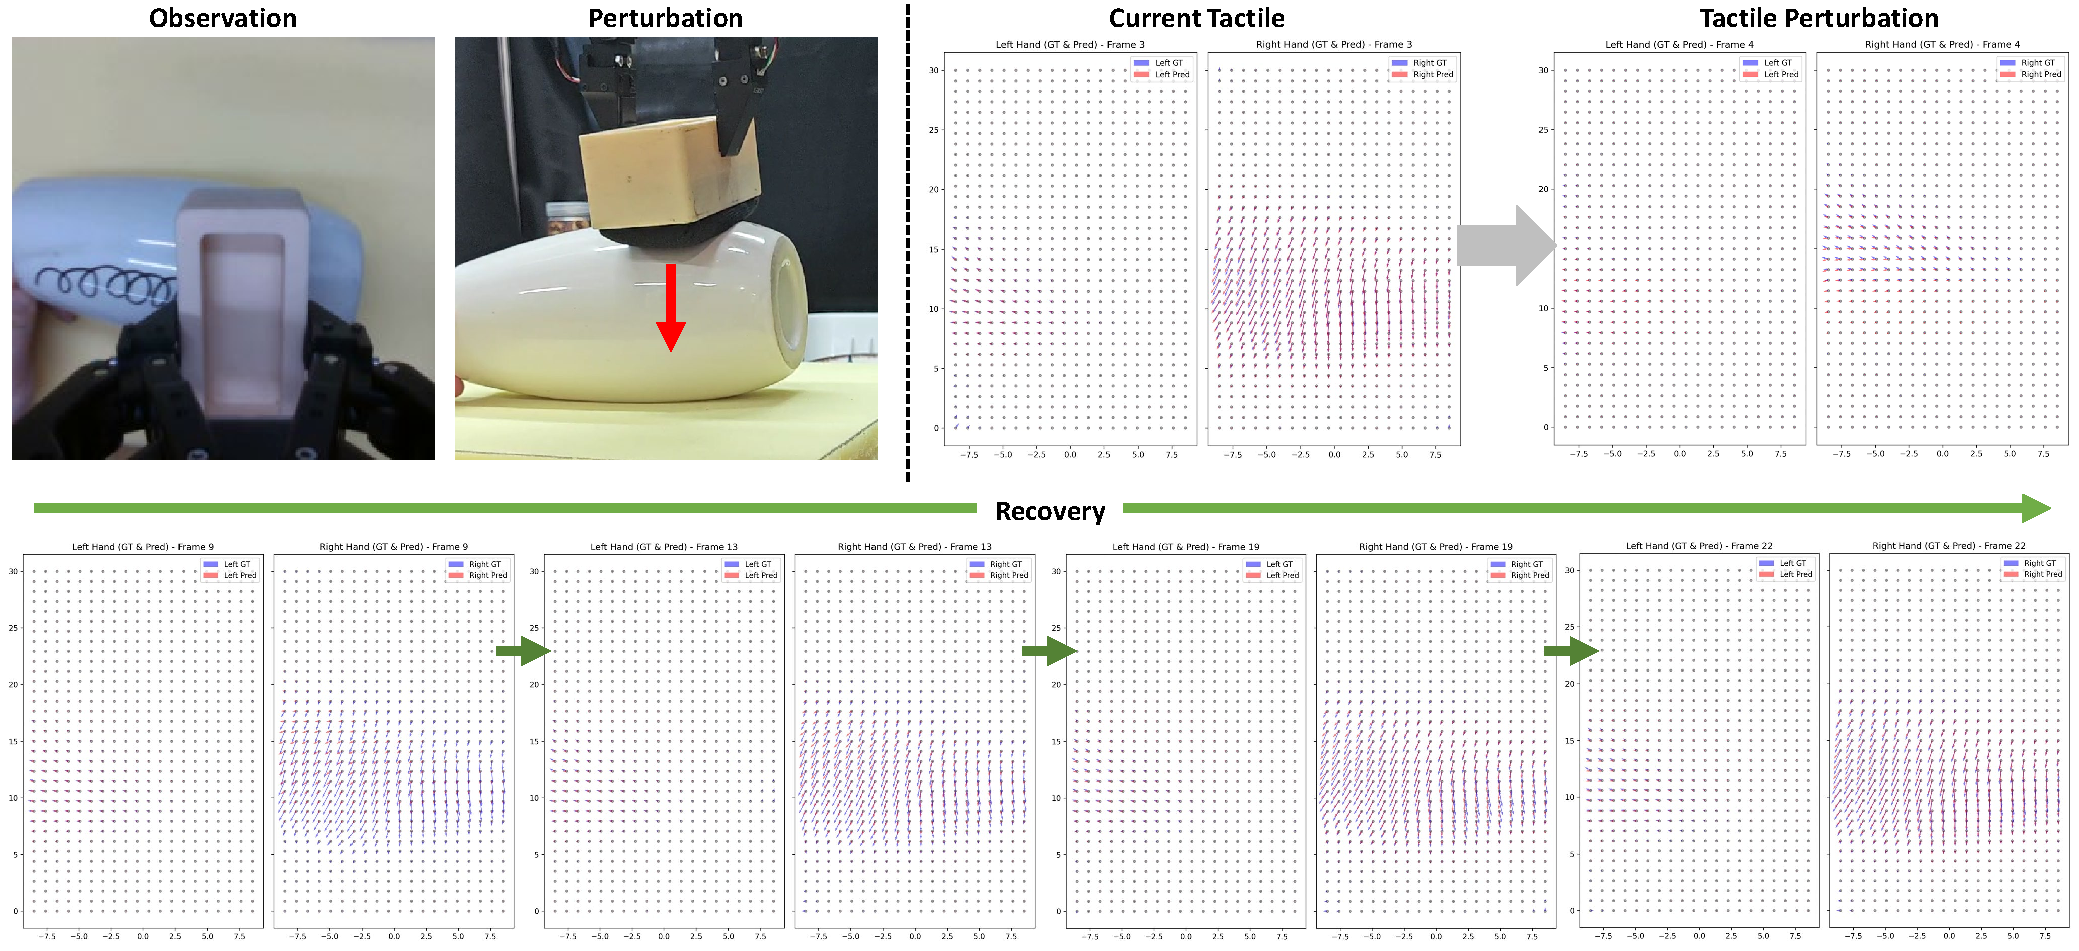
\includegraphics[width=0.95\linewidth]{fig/wm_disturb.pdf}
\caption{\textbf{Perturbation and recovery.} The first row shows a contact break due to downward perturbation, with tactile signals transitioning to a no-contact state. The second row shows recovery to the contact state within one generation chunk. In tactile visualization, red arrows denote tactile prediction while blue arrows denote ground truth.}
\label{fig:wm_disturb}
\vspace{-3mm}
\end{figure*}

\subsubsection{Adaptive Visuo-Tactile Fusion Policy}

In this section, we analyze the key components of the proposed Adaptive Visuo-Tactile Fusion Policy through a series of experiments and address the following questions:
(1) Does predicted future tactile information improve action planning?
(2) Is the proposed Latent Tactile Differential (LTD) Encoder more effective than simple feature concatenation?
(3) Is the gating mechanism necessary for adaptive visuo-tactile fusion, and do modality weights correlate with contact states?
(4) Does the Visuo-Tactile Diffusion Policy depend on the accuracy of tactile prediction?
(5) Do generated visual features further improve policy performance?
(6) What role does the Reflexive Latent Tactile Controller play during execution?

\noindent \textbf{Effect of predicted tactile signals.}
We first investigate whether predicted tactile information improves action planning. As shown in Table~\ref{tab:ablation_components_scaled}, we compare two tactile representations:
(1) using only the current tactile observation, and
(2) concatenating the current tactile observation with predicted tactile features at future horizons of 2, 4, and 6 steps.
To eliminate the influence of feature dimensionality, the concatenated tactile features are projected to the same dimension as the current tactile representation through a linear layer, ensuring consistent policy input size across settings. 
In this experiment, the gating mechanism is retained while the controller is disabled.
Results show that incorporating predicted tactile information consistently improves policy success rates, and longer prediction horizons (6 steps) outperform shorter ones (4 steps and 2 steps). This indicates that future tactile prediction provides richer contact dynamics that benefit action planning.

\begin{table}[t]
\centering
\caption{Ablation study on Adaptive Visuo-Tactile Fusion Policy and the components' impact on task success rate.}
\label{tab:ablation_components_scaled}
\small
\setlength{\tabcolsep}{6pt}
\renewcommand{\arraystretch}{1.2}

\begin{tabular}{ccccccc}
\toprule
\multicolumn{4}{c}{\textbf{Component}} & \multicolumn{3}{c}{\textbf{Success Rate}} \\
\cmidrule(lr){1-4} \cmidrule(lr){5-7}
\begin{tabular}[c]{@{}c@{}}Tactile Pred.\\ Length\end{tabular} & LTD & \begin{tabular}[c]{@{}c@{}}Gating\\ Mech.\end{tabular} & \begin{tabular}[c]{@{}c@{}}Visual\\ Gen.\end{tabular} & Wipe & Peel & Avg. \\
\midrule
0 & $\times$ & $\times$ & $\times$ & 0.12 & 0.06 & 0.09 \\
2 & $\times$ & $\times$ & $\times$ & 0.40 & 0.26 & 0.33 \\
4 & $\times$ & $\times$ & $\times$ & 0.45 & 0.30 & 0.38 \\
6 & $\times$ & $\times$ & $\times$ & 0.50 & 0.30 & 0.40 \\
\midrule
6 & \checkmark & $\times$ & $\times$ & 0.57 & 0.36 & 0.47 \\
6 & \checkmark & \checkmark & $\times$ & 0.66 & \textbf{0.40} & 0.53 \\
6 & \checkmark & \checkmark & \checkmark & \textbf{0.70} & 0.38 & \textbf{0.54} \\
\bottomrule
\end{tabular}
\end{table}
\begin{table}[t]
\centering
\caption{Inference time of each component on RTX 4090D.}
\label{tab:policy_time}
\small
\setlength{\tabcolsep}{8pt} % 增加列间距，避免表头太挤
\renewcommand{\arraystretch}{1.3}
\resizebox{0.9\linewidth}{!}{
\begin{tabular}{c c c} % 使用siunitx对齐数字
\toprule
 Slow Policy & Slow Policy w/ Visual Gen. & Fast Policy \\
\midrule
 230 ms & 480 ms & 3.5 ms \\
\bottomrule
\end{tabular}
}
\end{table}

\noindent \textbf{Comparison of tactile representations.}
We further compare different tactile representation strategies:
(1) direct concatenation of current and predicted tactile features, and
(2) the proposed LTD Encoder applied to both signals.
For fair comparison, the resulting tactile features are projected to the same dimensionality before being fed into the policy network.
As shown in Table~\ref{tab:ablation_components_scaled}, the LTD-based representation achieves higher success rates across multiple tasks. This suggests that the LTD Encoder effectively captures the dynamic relationship between current and predicted tactile, producing a more informative tactile representation for policy learning.

\begin{figure*}[t]
\centering
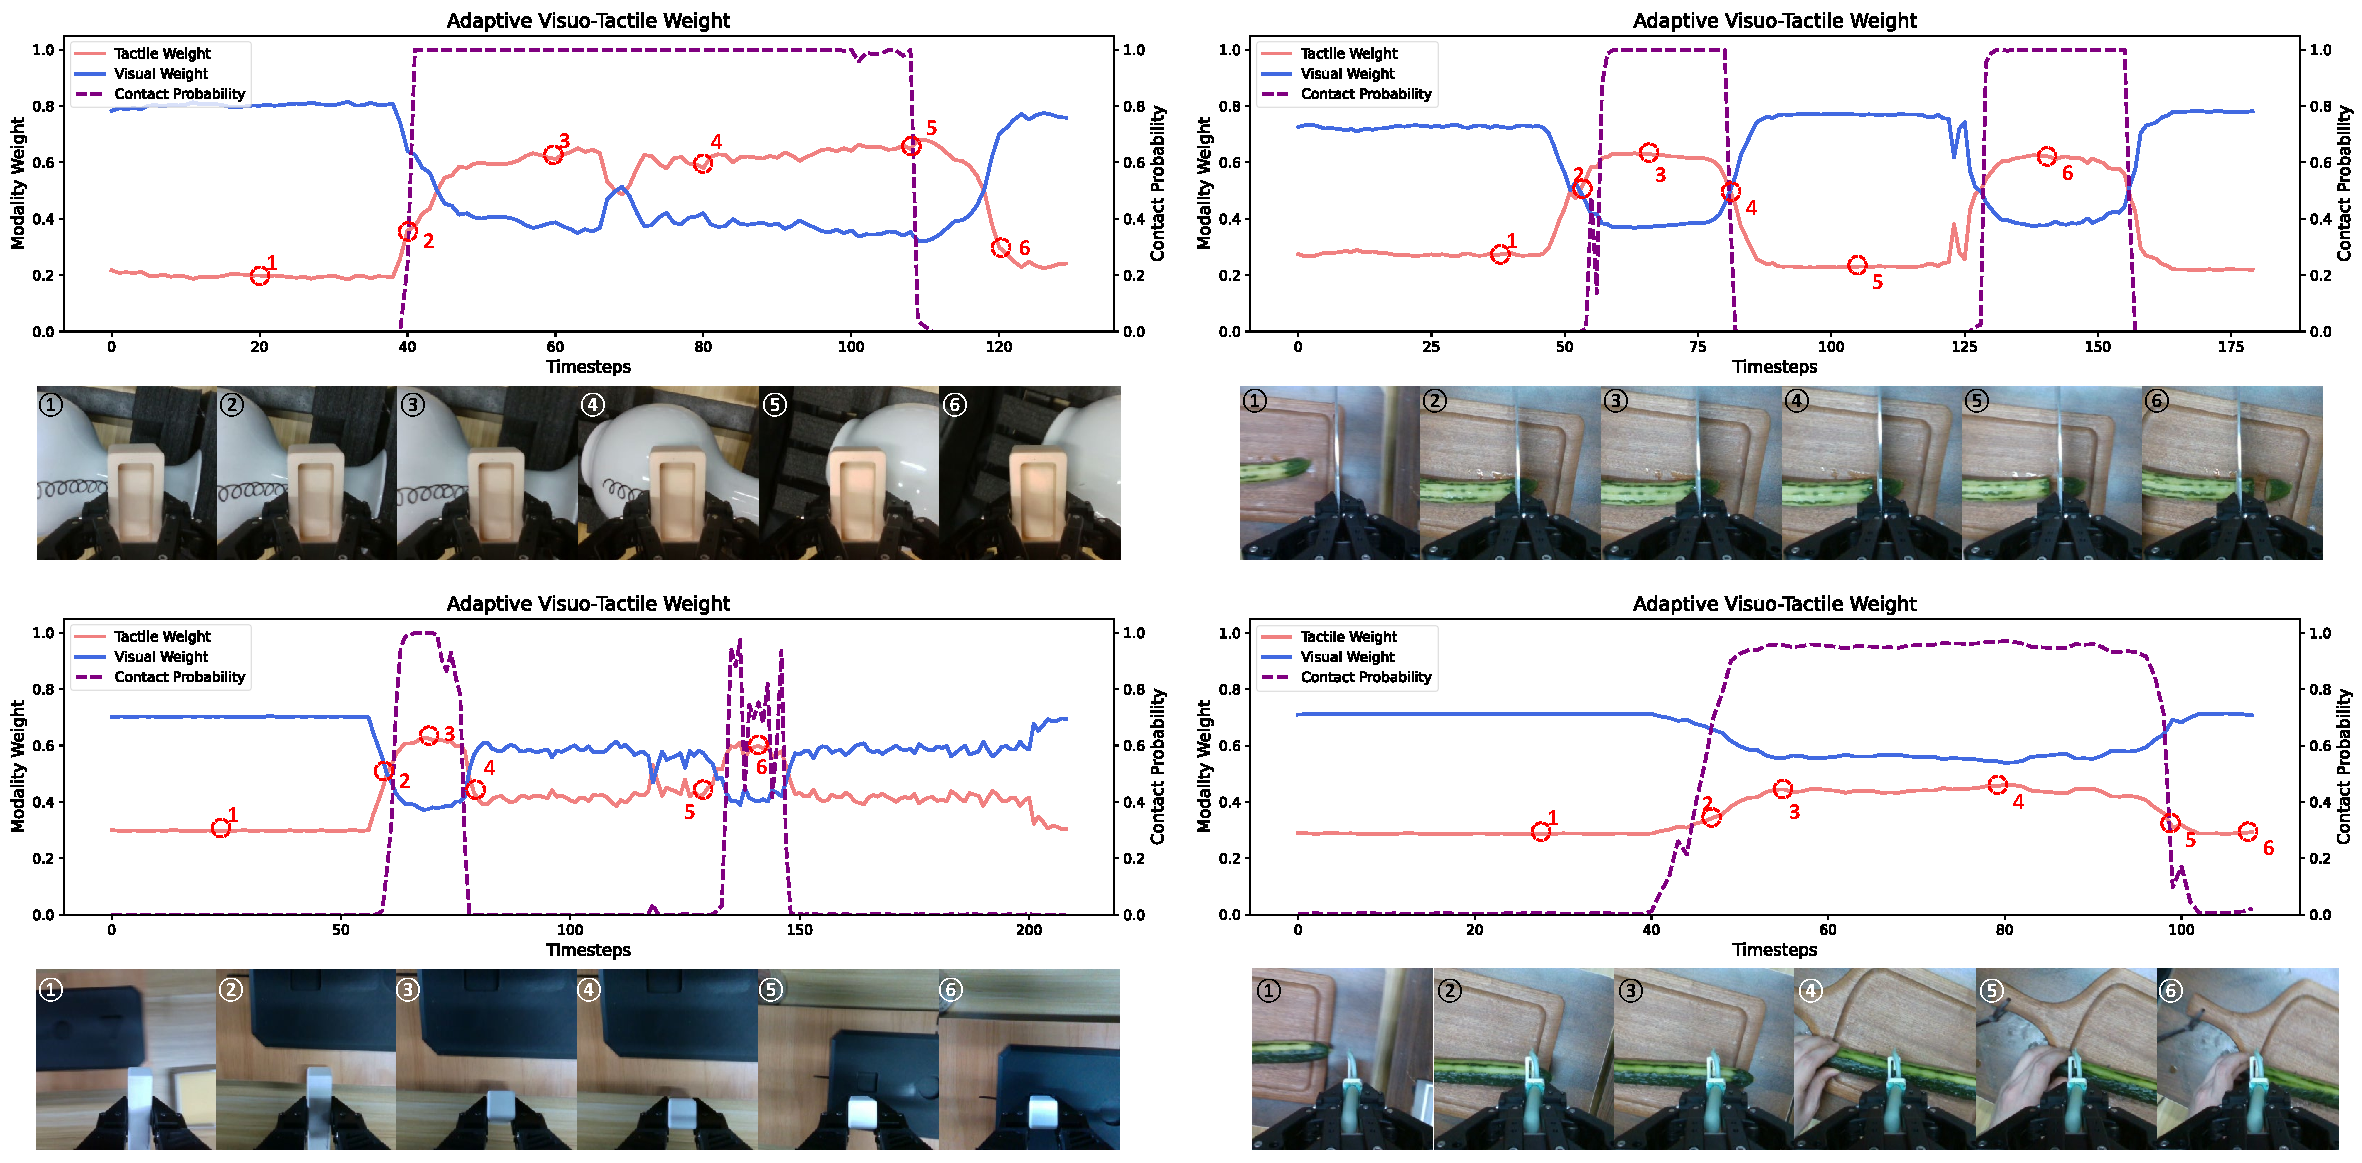
\includegraphics[width=0.95\linewidth]{fig/gate_weight.pdf}
\caption{G\textbf{Gating Fusion Mechanism.} We visualize the temporal evolution of the predicted contact probability (purple), together with the corresponding visual (blue) and tactile (red) weights over the course of task execution.}
\label{fig:gate_weight}
\vspace{-3mm}
\end{figure*}

\begin{figure*}[ht]
\centering
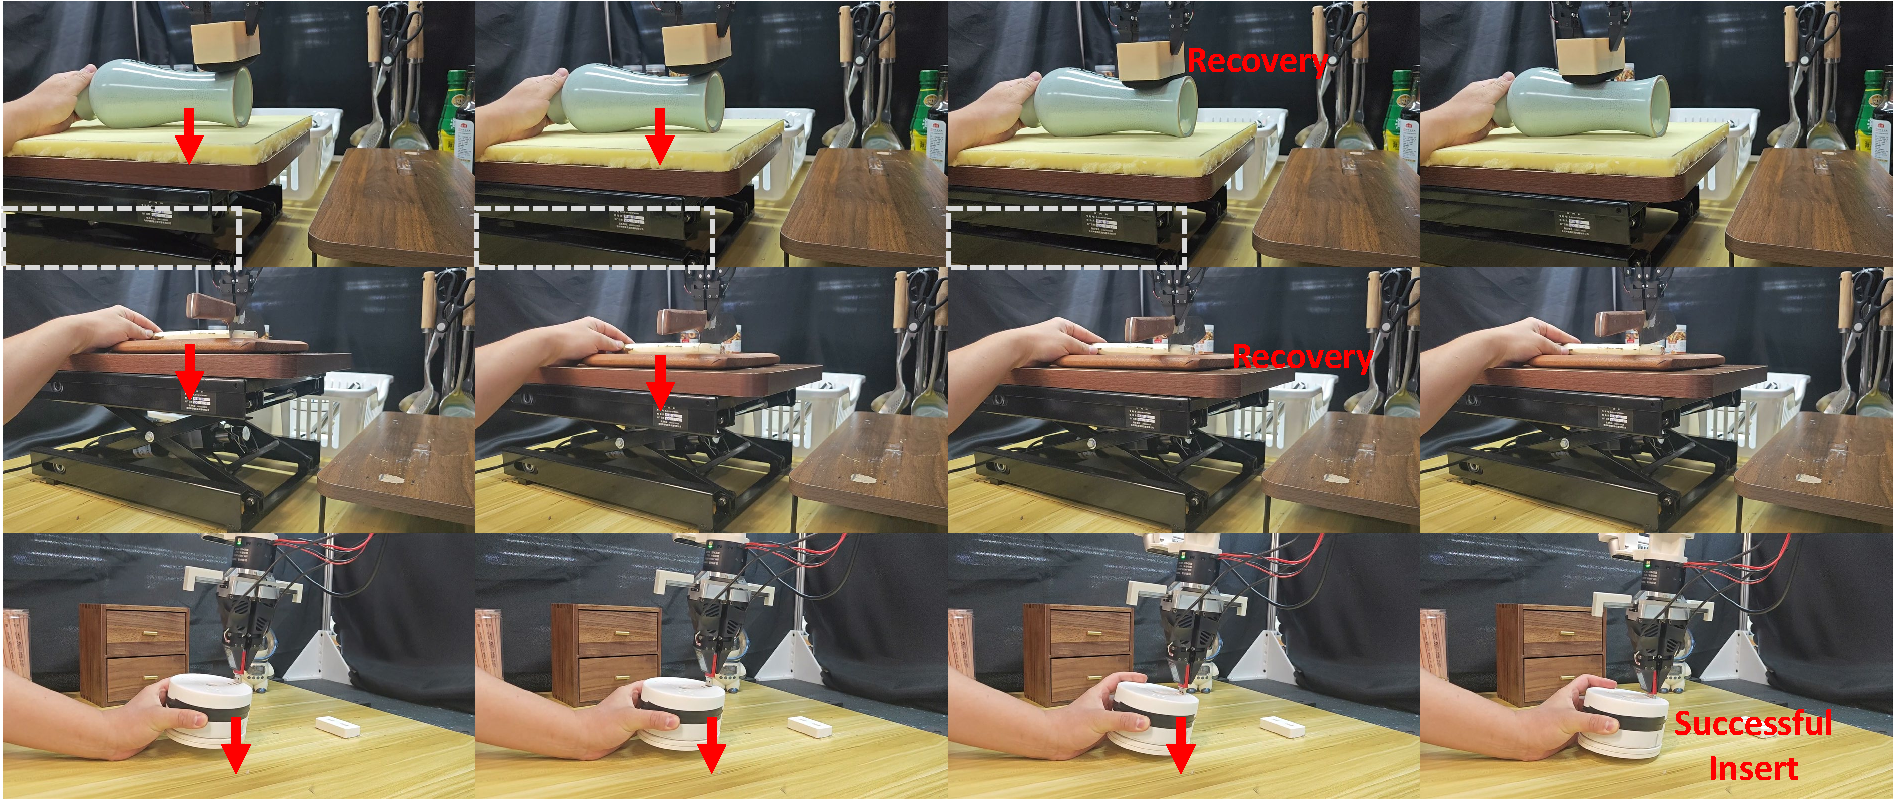
\includegraphics[width=0.95\linewidth]{fig/mp_disturb.pdf}
\caption{\textbf{Perturbation experiments.} We break contact by abruptly lowering the object and demonstrate how the policy rapidly restores contact via the RLTC.}
\label{fig:mp_disturb}
\vspace{-3mm}
\end{figure*}


\noindent \textbf{Necessity of the gating fusion mechanism.}
Next, we evaluate the effectiveness of the gating mechanism for visuo-tactile fusion by comparing two input configurations:
(1) direct concatenation of visual features and LTD-encoded tactile features, and
(2) adaptive fusion using the proposed gating mechanism.
As shown in Table~\ref{tab:ablation_components_scaled}, the gating mechanism improves the average task success rate by approximately 7\% compared to direct concatenation.
We further visualize the predicted contact probability and the modality weights in Fig.~\ref{fig:gate_weight}.
The results show a strong correlation between modality weights and contact states: when no contact occurs, the tactile weight remains close to zero, while it increases significantly as the predicted contact probability rises, indicating that action planning increasingly relies on tactile information during contact.

\noindent \textbf{Effect of tactile prediction.}
To evaluate how policy performance depends on tactile prediction quality, we introduce controlled prediction errors by using world model checkpoints with varying tactile prediction accuracies, corresponding to 80\%, 60\%, 40\%, and 20\% of the performance of the best-performing model.
As shown in Fig.~\ref{fig:prediction}, as prediction accuracy decreases, the policy gradually loses its ability to correctly infer contact states and adjust modality weights, leading to degraded action planning performance. This proves that accurate tactile prediction plays a critical role in our policy.

\begin{figure}[ht]
\centering
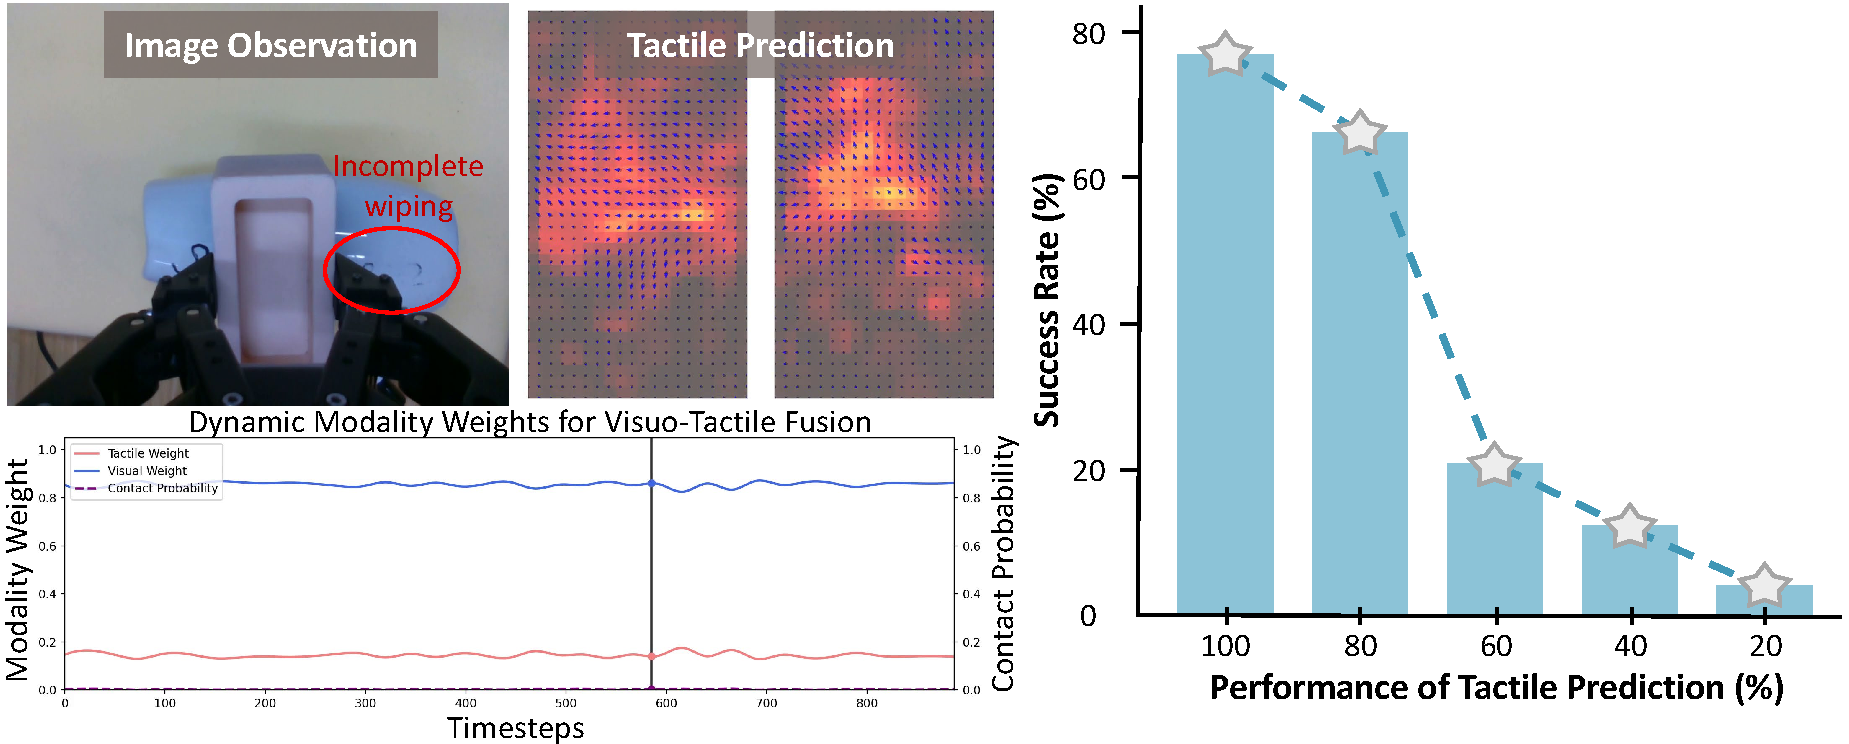
\includegraphics[width=\linewidth]{fig/prediction.pdf}
\caption{\textbf{Effect of tactile prediction accuracy.} \textbf{Left:} At 60\% prediction performance, the model fails to estimate future contact probability, resulting in improper modality weighting. \textbf{Right:} Lower prediction performance leads to a significant drop in success rate.}
\label{fig:prediction}
\vspace{-5mm}
\end{figure}

\noindent \textbf{Effect of generated visual features.}
We also investigate whether incorporating generated visual features improves policy performance.
Experimental results show that adding generated visual features to the policy input does not yield significant performance gains, as shown in Table~\ref{tab:ablation_components_scaled}. Moreover, introducing a visual generation branch significantly reduces inference frequency, as shown in Table~\ref{tab:policy_time}. Therefore, the final policy design relies only on current visual observations rather than on the generation.

\noindent \textbf{Effectiveness of the Reflexive Latent Tactile Controller.}
Finally, we evaluate the contribution of the Reflexive Latent Tactile Controller.
The controller enables high-frequency closed-loop control, allowing the robot to execute actions more stably and improving overall task success rates.
In perturbation experiments, shown in Table~\ref{tab:full_comparison_final_scaled} and Fig.~\ref{fig:mp_disturb}, the controller rapidly responds to environmental perturbations. When perturbations disrupt the current contact state, the high-frequency controller adjusts robot actions to re-establish stable contact.
In tasks requiring strong interaction forces, the controller also adaptively modulates the action magnitude to prevent excessive contact forces.

